% Created by tikzDevice version 0.12.3.1 on 2020-12-15 14:58:40
% !TEX encoding = UTF-8 Unicode
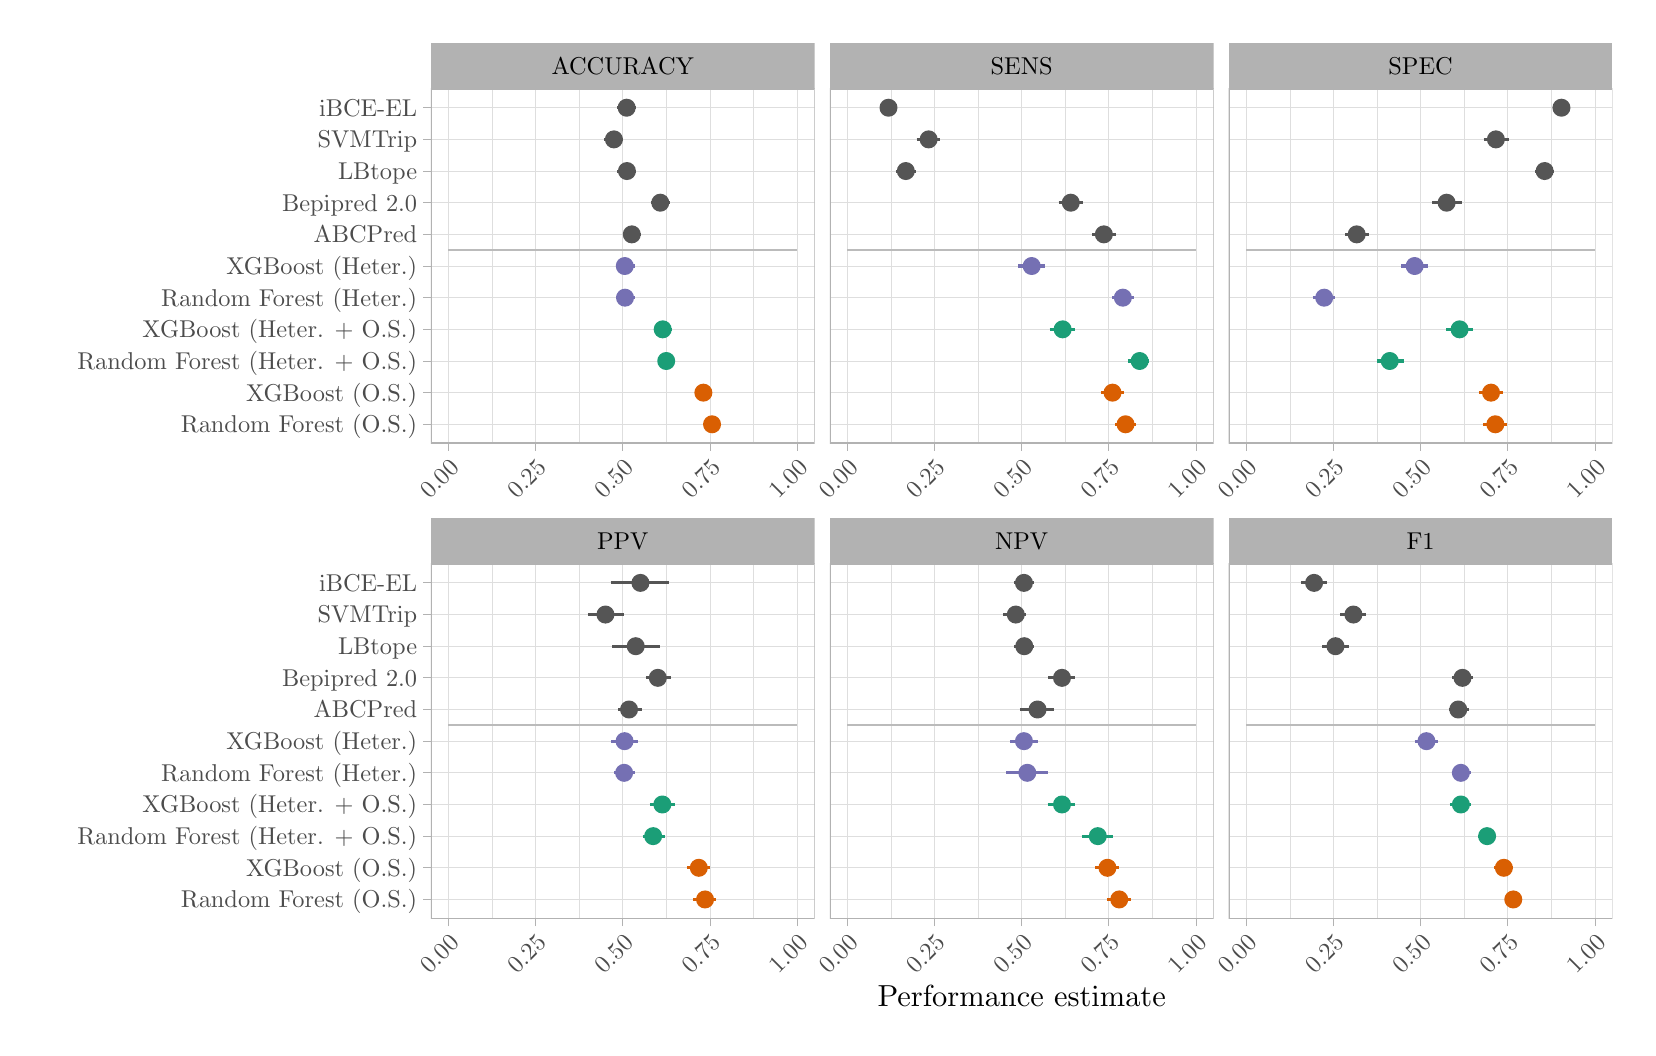
\begin{tikzpicture}[x=1pt,y=1pt]
\definecolor{fillColor}{RGB}{255,255,255}
\path[use as bounding box,fill=fillColor,fill opacity=0.00] (0,0) rectangle (578.16,361.35);
\begin{scope}
\path[clip] (  0.00,  0.00) rectangle (578.16,361.35);
\definecolor{drawColor}{RGB}{255,255,255}
\definecolor{fillColor}{RGB}{255,255,255}

\path[draw=drawColor,line width= 0.6pt,line join=round,line cap=round,fill=fillColor] (  0.00,  0.00) rectangle (578.16,361.35);
\end{scope}
\begin{scope}
\path[clip] (145.69,211.16) rectangle (284.35,339.28);
\definecolor{fillColor}{RGB}{255,255,255}

\path[fill=fillColor] (145.69,211.16) rectangle (284.35,339.28);
\definecolor{drawColor}{gray}{0.87}

\path[draw=drawColor,line width= 0.1pt,line join=round] (167.75,211.16) --
	(167.75,339.28);

\path[draw=drawColor,line width= 0.1pt,line join=round] (199.27,211.16) --
	(199.27,339.28);

\path[draw=drawColor,line width= 0.1pt,line join=round] (230.78,211.16) --
	(230.78,339.28);

\path[draw=drawColor,line width= 0.1pt,line join=round] (262.29,211.16) --
	(262.29,339.28);

\path[draw=drawColor,line width= 0.3pt,line join=round] (145.69,218.03) --
	(284.35,218.03);

\path[draw=drawColor,line width= 0.3pt,line join=round] (145.69,229.46) --
	(284.35,229.46);

\path[draw=drawColor,line width= 0.3pt,line join=round] (145.69,240.90) --
	(284.35,240.90);

\path[draw=drawColor,line width= 0.3pt,line join=round] (145.69,252.34) --
	(284.35,252.34);

\path[draw=drawColor,line width= 0.3pt,line join=round] (145.69,263.78) --
	(284.35,263.78);

\path[draw=drawColor,line width= 0.3pt,line join=round] (145.69,275.22) --
	(284.35,275.22);

\path[draw=drawColor,line width= 0.3pt,line join=round] (145.69,286.66) --
	(284.35,286.66);

\path[draw=drawColor,line width= 0.3pt,line join=round] (145.69,298.10) --
	(284.35,298.10);

\path[draw=drawColor,line width= 0.3pt,line join=round] (145.69,309.54) --
	(284.35,309.54);

\path[draw=drawColor,line width= 0.3pt,line join=round] (145.69,320.98) --
	(284.35,320.98);

\path[draw=drawColor,line width= 0.3pt,line join=round] (145.69,332.42) --
	(284.35,332.42);

\path[draw=drawColor,line width= 0.3pt,line join=round] (152.00,211.16) --
	(152.00,339.28);

\path[draw=drawColor,line width= 0.3pt,line join=round] (183.51,211.16) --
	(183.51,339.28);

\path[draw=drawColor,line width= 0.3pt,line join=round] (215.02,211.16) --
	(215.02,339.28);

\path[draw=drawColor,line width= 0.3pt,line join=round] (246.53,211.16) --
	(246.53,339.28);

\path[draw=drawColor,line width= 0.3pt,line join=round] (278.05,211.16) --
	(278.05,339.28);
\definecolor{drawColor}{RGB}{217,95,2}

\path[draw=drawColor,line width= 1.1pt,line join=round] (244.25,218.03) -- (250.13,218.03);

\path[draw=drawColor,line width= 1.1pt,line join=round] (241.12,229.46) -- (247.10,229.46);
\definecolor{drawColor}{RGB}{27,158,119}

\path[draw=drawColor,line width= 1.1pt,line join=round] (227.61,240.90) -- (233.97,240.90);

\path[draw=drawColor,line width= 1.1pt,line join=round] (226.14,252.34) -- (232.90,252.34);
\definecolor{drawColor}{RGB}{117,112,179}

\path[draw=drawColor,line width= 1.1pt,line join=round] (212.72,263.78) -- (219.38,263.78);

\path[draw=drawColor,line width= 1.1pt,line join=round] (212.52,275.22) -- (219.28,275.22);
\definecolor{drawColor}{RGB}{85,85,85}

\path[draw=drawColor,line width= 1.1pt,line join=round] (215.07,286.66) -- (221.74,286.66);

\path[draw=drawColor,line width= 1.1pt,line join=round] (225.16,298.10) -- (232.21,298.10);

\path[draw=drawColor,line width= 1.1pt,line join=round] (213.11,309.54) -- (219.97,309.54);

\path[draw=drawColor,line width= 1.1pt,line join=round] (208.21,320.98) -- (215.27,320.98);

\path[draw=drawColor,line width= 1.1pt,line join=round] (213.11,332.42) -- (219.77,332.42);
\definecolor{drawColor}{RGB}{217,95,2}
\definecolor{fillColor}{RGB}{217,95,2}

\path[draw=drawColor,line width= 0.8pt,line join=round,line cap=round,fill=fillColor] (247.29,218.03) circle (  2.85);

\path[draw=drawColor,line width= 0.8pt,line join=round,line cap=round,fill=fillColor] (244.16,229.46) circle (  2.85);
\definecolor{drawColor}{RGB}{27,158,119}
\definecolor{fillColor}{RGB}{27,158,119}

\path[draw=drawColor,line width= 0.8pt,line join=round,line cap=round,fill=fillColor] (230.74,240.90) circle (  2.85);

\path[draw=drawColor,line width= 0.8pt,line join=round,line cap=round,fill=fillColor] (229.47,252.34) circle (  2.85);
\definecolor{drawColor}{RGB}{117,112,179}
\definecolor{fillColor}{RGB}{117,112,179}

\path[draw=drawColor,line width= 0.8pt,line join=round,line cap=round,fill=fillColor] (215.85,263.78) circle (  2.85);

\path[draw=drawColor,line width= 0.8pt,line join=round,line cap=round,fill=fillColor] (215.76,275.22) circle (  2.85);
\definecolor{drawColor}{RGB}{85,85,85}
\definecolor{fillColor}{RGB}{85,85,85}

\path[draw=drawColor,line width= 0.8pt,line join=round,line cap=round,fill=fillColor] (218.30,286.66) circle (  2.85);

\path[draw=drawColor,line width= 0.8pt,line join=round,line cap=round,fill=fillColor] (228.59,298.10) circle (  2.85);

\path[draw=drawColor,line width= 0.8pt,line join=round,line cap=round,fill=fillColor] (216.54,309.54) circle (  2.85);

\path[draw=drawColor,line width= 0.8pt,line join=round,line cap=round,fill=fillColor] (211.84,320.98) circle (  2.85);

\path[draw=drawColor,line width= 0.8pt,line join=round,line cap=round,fill=fillColor] (216.44,332.42) circle (  2.85);
\definecolor{drawColor}{RGB}{187,187,187}

\path[draw=drawColor,line width= 0.6pt,line join=round] (152.00,280.94) -- (278.05,280.94);
\definecolor{drawColor}{gray}{0.70}

\path[draw=drawColor,line width= 0.6pt,line join=round,line cap=round] (145.69,211.16) rectangle (284.35,339.28);
\end{scope}
\begin{scope}
\path[clip] (145.69, 39.47) rectangle (284.35,167.59);
\definecolor{fillColor}{RGB}{255,255,255}

\path[fill=fillColor] (145.69, 39.47) rectangle (284.35,167.59);
\definecolor{drawColor}{gray}{0.87}

\path[draw=drawColor,line width= 0.1pt,line join=round] (167.75, 39.47) --
	(167.75,167.59);

\path[draw=drawColor,line width= 0.1pt,line join=round] (199.27, 39.47) --
	(199.27,167.59);

\path[draw=drawColor,line width= 0.1pt,line join=round] (230.78, 39.47) --
	(230.78,167.59);

\path[draw=drawColor,line width= 0.1pt,line join=round] (262.29, 39.47) --
	(262.29,167.59);

\path[draw=drawColor,line width= 0.3pt,line join=round] (145.69, 46.33) --
	(284.35, 46.33);

\path[draw=drawColor,line width= 0.3pt,line join=round] (145.69, 57.77) --
	(284.35, 57.77);

\path[draw=drawColor,line width= 0.3pt,line join=round] (145.69, 69.21) --
	(284.35, 69.21);

\path[draw=drawColor,line width= 0.3pt,line join=round] (145.69, 80.65) --
	(284.35, 80.65);

\path[draw=drawColor,line width= 0.3pt,line join=round] (145.69, 92.09) --
	(284.35, 92.09);

\path[draw=drawColor,line width= 0.3pt,line join=round] (145.69,103.53) --
	(284.35,103.53);

\path[draw=drawColor,line width= 0.3pt,line join=round] (145.69,114.97) --
	(284.35,114.97);

\path[draw=drawColor,line width= 0.3pt,line join=round] (145.69,126.41) --
	(284.35,126.41);

\path[draw=drawColor,line width= 0.3pt,line join=round] (145.69,137.84) --
	(284.35,137.84);

\path[draw=drawColor,line width= 0.3pt,line join=round] (145.69,149.28) --
	(284.35,149.28);

\path[draw=drawColor,line width= 0.3pt,line join=round] (145.69,160.72) --
	(284.35,160.72);

\path[draw=drawColor,line width= 0.3pt,line join=round] (152.00, 39.47) --
	(152.00,167.59);

\path[draw=drawColor,line width= 0.3pt,line join=round] (183.51, 39.47) --
	(183.51,167.59);

\path[draw=drawColor,line width= 0.3pt,line join=round] (215.02, 39.47) --
	(215.02,167.59);

\path[draw=drawColor,line width= 0.3pt,line join=round] (246.53, 39.47) --
	(246.53,167.59);

\path[draw=drawColor,line width= 0.3pt,line join=round] (278.05, 39.47) --
	(278.05,167.59);
\definecolor{drawColor}{RGB}{217,95,2}

\path[draw=drawColor,line width= 1.1pt,line join=round] (240.55, 46.33) -- (248.89, 46.33);

\path[draw=drawColor,line width= 1.1pt,line join=round] (238.17, 57.77) -- (246.68, 57.77);
\definecolor{drawColor}{RGB}{27,158,119}

\path[draw=drawColor,line width= 1.1pt,line join=round] (222.20, 69.21) -- (230.21, 69.21);

\path[draw=drawColor,line width= 1.1pt,line join=round] (224.79, 80.65) -- (234.00, 80.65);
\definecolor{drawColor}{RGB}{117,112,179}

\path[draw=drawColor,line width= 1.1pt,line join=round] (211.92, 92.09) -- (219.62, 92.09);

\path[draw=drawColor,line width= 1.1pt,line join=round] (210.92,103.53) -- (220.36,103.53);
\definecolor{drawColor}{RGB}{85,85,85}

\path[draw=drawColor,line width= 1.1pt,line join=round] (213.37,114.97) -- (221.89,114.97);

\path[draw=drawColor,line width= 1.1pt,line join=round] (223.38,126.41) -- (232.38,126.41);

\path[draw=drawColor,line width= 1.1pt,line join=round] (211.22,137.84) -- (228.64,137.84);

\path[draw=drawColor,line width= 1.1pt,line join=round] (202.41,149.28) -- (215.62,149.28);

\path[draw=drawColor,line width= 1.1pt,line join=round] (210.69,160.72) -- (231.61,160.72);
\definecolor{drawColor}{RGB}{217,95,2}
\definecolor{fillColor}{RGB}{217,95,2}

\path[draw=drawColor,line width= 0.8pt,line join=round,line cap=round,fill=fillColor] (244.77, 46.33) circle (  2.85);

\path[draw=drawColor,line width= 0.8pt,line join=round,line cap=round,fill=fillColor] (242.51, 57.77) circle (  2.85);
\definecolor{drawColor}{RGB}{27,158,119}
\definecolor{fillColor}{RGB}{27,158,119}

\path[draw=drawColor,line width= 0.8pt,line join=round,line cap=round,fill=fillColor] (226.01, 69.21) circle (  2.85);

\path[draw=drawColor,line width= 0.8pt,line join=round,line cap=round,fill=fillColor] (229.34, 80.65) circle (  2.85);
\definecolor{drawColor}{RGB}{117,112,179}
\definecolor{fillColor}{RGB}{117,112,179}

\path[draw=drawColor,line width= 0.8pt,line join=round,line cap=round,fill=fillColor] (215.52, 92.09) circle (  2.85);

\path[draw=drawColor,line width= 0.8pt,line join=round,line cap=round,fill=fillColor] (215.68,103.53) circle (  2.85);
\definecolor{drawColor}{RGB}{85,85,85}
\definecolor{fillColor}{RGB}{85,85,85}

\path[draw=drawColor,line width= 0.8pt,line join=round,line cap=round,fill=fillColor] (217.30,114.97) circle (  2.85);

\path[draw=drawColor,line width= 0.8pt,line join=round,line cap=round,fill=fillColor] (227.70,126.41) circle (  2.85);

\path[draw=drawColor,line width= 0.8pt,line join=round,line cap=round,fill=fillColor] (219.72,137.84) circle (  2.85);

\path[draw=drawColor,line width= 0.8pt,line join=round,line cap=round,fill=fillColor] (208.78,149.28) circle (  2.85);

\path[draw=drawColor,line width= 0.8pt,line join=round,line cap=round,fill=fillColor] (221.42,160.72) circle (  2.85);
\definecolor{drawColor}{RGB}{187,187,187}

\path[draw=drawColor,line width= 0.6pt,line join=round] (152.00,109.25) -- (278.05,109.25);
\definecolor{drawColor}{gray}{0.70}

\path[draw=drawColor,line width= 0.6pt,line join=round,line cap=round] (145.69, 39.47) rectangle (284.35,167.59);
\end{scope}
\begin{scope}
\path[clip] (289.85,211.16) rectangle (428.50,339.28);
\definecolor{fillColor}{RGB}{255,255,255}

\path[fill=fillColor] (289.85,211.16) rectangle (428.50,339.28);
\definecolor{drawColor}{gray}{0.87}

\path[draw=drawColor,line width= 0.1pt,line join=round] (311.91,211.16) --
	(311.91,339.28);

\path[draw=drawColor,line width= 0.1pt,line join=round] (343.42,211.16) --
	(343.42,339.28);

\path[draw=drawColor,line width= 0.1pt,line join=round] (374.93,211.16) --
	(374.93,339.28);

\path[draw=drawColor,line width= 0.1pt,line join=round] (406.45,211.16) --
	(406.45,339.28);

\path[draw=drawColor,line width= 0.3pt,line join=round] (289.85,218.03) --
	(428.50,218.03);

\path[draw=drawColor,line width= 0.3pt,line join=round] (289.85,229.46) --
	(428.50,229.46);

\path[draw=drawColor,line width= 0.3pt,line join=round] (289.85,240.90) --
	(428.50,240.90);

\path[draw=drawColor,line width= 0.3pt,line join=round] (289.85,252.34) --
	(428.50,252.34);

\path[draw=drawColor,line width= 0.3pt,line join=round] (289.85,263.78) --
	(428.50,263.78);

\path[draw=drawColor,line width= 0.3pt,line join=round] (289.85,275.22) --
	(428.50,275.22);

\path[draw=drawColor,line width= 0.3pt,line join=round] (289.85,286.66) --
	(428.50,286.66);

\path[draw=drawColor,line width= 0.3pt,line join=round] (289.85,298.10) --
	(428.50,298.10);

\path[draw=drawColor,line width= 0.3pt,line join=round] (289.85,309.54) --
	(428.50,309.54);

\path[draw=drawColor,line width= 0.3pt,line join=round] (289.85,320.98) --
	(428.50,320.98);

\path[draw=drawColor,line width= 0.3pt,line join=round] (289.85,332.42) --
	(428.50,332.42);

\path[draw=drawColor,line width= 0.3pt,line join=round] (296.15,211.16) --
	(296.15,339.28);

\path[draw=drawColor,line width= 0.3pt,line join=round] (327.66,211.16) --
	(327.66,339.28);

\path[draw=drawColor,line width= 0.3pt,line join=round] (359.18,211.16) --
	(359.18,339.28);

\path[draw=drawColor,line width= 0.3pt,line join=round] (390.69,211.16) --
	(390.69,339.28);

\path[draw=drawColor,line width= 0.3pt,line join=round] (422.20,211.16) --
	(422.20,339.28);
\definecolor{drawColor}{RGB}{217,95,2}

\path[draw=drawColor,line width= 1.1pt,line join=round] (393.05,218.03) -- (400.63,218.03);

\path[draw=drawColor,line width= 1.1pt,line join=round] (387.97,229.46) -- (396.02,229.46);
\definecolor{drawColor}{RGB}{27,158,119}

\path[draw=drawColor,line width= 1.1pt,line join=round] (397.56,240.90) -- (405.27,240.90);

\path[draw=drawColor,line width= 1.1pt,line join=round] (369.28,252.34) -- (378.62,252.34);
\definecolor{drawColor}{RGB}{117,112,179}

\path[draw=drawColor,line width= 1.1pt,line join=round] (391.89,263.78) -- (399.84,263.78);

\path[draw=drawColor,line width= 1.1pt,line join=round] (357.85,275.22) -- (367.78,275.22);
\definecolor{drawColor}{RGB}{85,85,85}

\path[draw=drawColor,line width= 1.1pt,line join=round] (384.73,286.66) -- (393.23,286.66);

\path[draw=drawColor,line width= 1.1pt,line join=round] (372.51,298.10) -- (381.32,298.10);

\path[draw=drawColor,line width= 1.1pt,line join=round] (313.71,309.54) -- (321.17,309.54);

\path[draw=drawColor,line width= 1.1pt,line join=round] (321.24,320.98) -- (329.74,320.98);

\path[draw=drawColor,line width= 1.1pt,line join=round] (308.00,332.42) -- (314.16,332.42);
\definecolor{drawColor}{RGB}{217,95,2}
\definecolor{fillColor}{RGB}{217,95,2}

\path[draw=drawColor,line width= 0.8pt,line join=round,line cap=round,fill=fillColor] (396.72,218.03) circle (  2.85);

\path[draw=drawColor,line width= 0.8pt,line join=round,line cap=round,fill=fillColor] (392.01,229.46) circle (  2.85);
\definecolor{drawColor}{RGB}{27,158,119}
\definecolor{fillColor}{RGB}{27,158,119}

\path[draw=drawColor,line width= 0.8pt,line join=round,line cap=round,fill=fillColor] (401.81,240.90) circle (  2.85);

\path[draw=drawColor,line width= 0.8pt,line join=round,line cap=round,fill=fillColor] (373.98,252.34) circle (  2.85);
\definecolor{drawColor}{RGB}{117,112,179}
\definecolor{fillColor}{RGB}{117,112,179}

\path[draw=drawColor,line width= 0.8pt,line join=round,line cap=round,fill=fillColor] (395.74,263.78) circle (  2.85);

\path[draw=drawColor,line width= 0.8pt,line join=round,line cap=round,fill=fillColor] (362.80,275.22) circle (  2.85);
\definecolor{drawColor}{RGB}{85,85,85}
\definecolor{fillColor}{RGB}{85,85,85}

\path[draw=drawColor,line width= 0.8pt,line join=round,line cap=round,fill=fillColor] (388.88,286.66) circle (  2.85);

\path[draw=drawColor,line width= 0.8pt,line join=round,line cap=round,fill=fillColor] (376.92,298.10) circle (  2.85);

\path[draw=drawColor,line width= 0.8pt,line join=round,line cap=round,fill=fillColor] (317.32,309.54) circle (  2.85);

\path[draw=drawColor,line width= 0.8pt,line join=round,line cap=round,fill=fillColor] (325.56,320.98) circle (  2.85);

\path[draw=drawColor,line width= 0.8pt,line join=round,line cap=round,fill=fillColor] (311.05,332.42) circle (  2.85);
\definecolor{drawColor}{RGB}{187,187,187}

\path[draw=drawColor,line width= 0.6pt,line join=round] (296.15,280.94) -- (422.20,280.94);
\definecolor{drawColor}{gray}{0.70}

\path[draw=drawColor,line width= 0.6pt,line join=round,line cap=round] (289.85,211.16) rectangle (428.50,339.28);
\end{scope}
\begin{scope}
\path[clip] (289.85, 39.47) rectangle (428.50,167.59);
\definecolor{fillColor}{RGB}{255,255,255}

\path[fill=fillColor] (289.85, 39.47) rectangle (428.50,167.59);
\definecolor{drawColor}{gray}{0.87}

\path[draw=drawColor,line width= 0.1pt,line join=round] (311.91, 39.47) --
	(311.91,167.59);

\path[draw=drawColor,line width= 0.1pt,line join=round] (343.42, 39.47) --
	(343.42,167.59);

\path[draw=drawColor,line width= 0.1pt,line join=round] (374.93, 39.47) --
	(374.93,167.59);

\path[draw=drawColor,line width= 0.1pt,line join=round] (406.45, 39.47) --
	(406.45,167.59);

\path[draw=drawColor,line width= 0.3pt,line join=round] (289.85, 46.33) --
	(428.50, 46.33);

\path[draw=drawColor,line width= 0.3pt,line join=round] (289.85, 57.77) --
	(428.50, 57.77);

\path[draw=drawColor,line width= 0.3pt,line join=round] (289.85, 69.21) --
	(428.50, 69.21);

\path[draw=drawColor,line width= 0.3pt,line join=round] (289.85, 80.65) --
	(428.50, 80.65);

\path[draw=drawColor,line width= 0.3pt,line join=round] (289.85, 92.09) --
	(428.50, 92.09);

\path[draw=drawColor,line width= 0.3pt,line join=round] (289.85,103.53) --
	(428.50,103.53);

\path[draw=drawColor,line width= 0.3pt,line join=round] (289.85,114.97) --
	(428.50,114.97);

\path[draw=drawColor,line width= 0.3pt,line join=round] (289.85,126.41) --
	(428.50,126.41);

\path[draw=drawColor,line width= 0.3pt,line join=round] (289.85,137.84) --
	(428.50,137.84);

\path[draw=drawColor,line width= 0.3pt,line join=round] (289.85,149.28) --
	(428.50,149.28);

\path[draw=drawColor,line width= 0.3pt,line join=round] (289.85,160.72) --
	(428.50,160.72);

\path[draw=drawColor,line width= 0.3pt,line join=round] (296.15, 39.47) --
	(296.15,167.59);

\path[draw=drawColor,line width= 0.3pt,line join=round] (327.66, 39.47) --
	(327.66,167.59);

\path[draw=drawColor,line width= 0.3pt,line join=round] (359.18, 39.47) --
	(359.18,167.59);

\path[draw=drawColor,line width= 0.3pt,line join=round] (390.69, 39.47) --
	(390.69,167.59);

\path[draw=drawColor,line width= 0.3pt,line join=round] (422.20, 39.47) --
	(422.20,167.59);
\definecolor{drawColor}{RGB}{217,95,2}

\path[draw=drawColor,line width= 1.1pt,line join=round] (389.98, 46.33) -- (398.61, 46.33);

\path[draw=drawColor,line width= 1.1pt,line join=round] (385.68, 57.77) -- (394.19, 57.77);
\definecolor{drawColor}{RGB}{27,158,119}

\path[draw=drawColor,line width= 1.1pt,line join=round] (380.86, 69.21) -- (392.19, 69.21);

\path[draw=drawColor,line width= 1.1pt,line join=round] (368.59, 80.65) -- (378.36, 80.65);
\definecolor{drawColor}{RGB}{117,112,179}

\path[draw=drawColor,line width= 1.1pt,line join=round] (353.64, 92.09) -- (368.52, 92.09);

\path[draw=drawColor,line width= 1.1pt,line join=round] (355.06,103.53) -- (365.01,103.53);
\definecolor{drawColor}{RGB}{85,85,85}

\path[draw=drawColor,line width= 1.1pt,line join=round] (358.51,114.97) -- (371.02,114.97);

\path[draw=drawColor,line width= 1.1pt,line join=round] (368.74,126.41) -- (378.50,126.41);

\path[draw=drawColor,line width= 1.1pt,line join=round] (356.33,137.84) -- (363.72,137.84);

\path[draw=drawColor,line width= 1.1pt,line join=round] (352.57,149.28) -- (360.84,149.28);

\path[draw=drawColor,line width= 1.1pt,line join=round] (356.36,160.72) -- (363.46,160.72);
\definecolor{drawColor}{RGB}{217,95,2}
\definecolor{fillColor}{RGB}{217,95,2}

\path[draw=drawColor,line width= 0.8pt,line join=round,line cap=round,fill=fillColor] (394.43, 46.33) circle (  2.85);

\path[draw=drawColor,line width= 0.8pt,line join=round,line cap=round,fill=fillColor] (390.17, 57.77) circle (  2.85);
\definecolor{drawColor}{RGB}{27,158,119}
\definecolor{fillColor}{RGB}{27,158,119}

\path[draw=drawColor,line width= 0.8pt,line join=round,line cap=round,fill=fillColor] (386.68, 69.21) circle (  2.85);

\path[draw=drawColor,line width= 0.8pt,line join=round,line cap=round,fill=fillColor] (373.75, 80.65) circle (  2.85);
\definecolor{drawColor}{RGB}{117,112,179}
\definecolor{fillColor}{RGB}{117,112,179}

\path[draw=drawColor,line width= 0.8pt,line join=round,line cap=round,fill=fillColor] (361.21, 92.09) circle (  2.85);

\path[draw=drawColor,line width= 0.8pt,line join=round,line cap=round,fill=fillColor] (360.00,103.53) circle (  2.85);
\definecolor{drawColor}{RGB}{85,85,85}
\definecolor{fillColor}{RGB}{85,85,85}

\path[draw=drawColor,line width= 0.8pt,line join=round,line cap=round,fill=fillColor] (364.91,114.97) circle (  2.85);

\path[draw=drawColor,line width= 0.8pt,line join=round,line cap=round,fill=fillColor] (373.75,126.41) circle (  2.85);

\path[draw=drawColor,line width= 0.8pt,line join=round,line cap=round,fill=fillColor] (360.11,137.84) circle (  2.85);

\path[draw=drawColor,line width= 0.8pt,line join=round,line cap=round,fill=fillColor] (357.06,149.28) circle (  2.85);

\path[draw=drawColor,line width= 0.8pt,line join=round,line cap=round,fill=fillColor] (360.00,160.72) circle (  2.85);
\definecolor{drawColor}{RGB}{187,187,187}

\path[draw=drawColor,line width= 0.6pt,line join=round] (296.15,109.25) -- (422.20,109.25);
\definecolor{drawColor}{gray}{0.70}

\path[draw=drawColor,line width= 0.6pt,line join=round,line cap=round] (289.85, 39.47) rectangle (428.50,167.59);
\end{scope}
\begin{scope}
\path[clip] (434.00,211.16) rectangle (572.66,339.28);
\definecolor{fillColor}{RGB}{255,255,255}

\path[fill=fillColor] (434.00,211.16) rectangle (572.66,339.28);
\definecolor{drawColor}{gray}{0.87}

\path[draw=drawColor,line width= 0.1pt,line join=round] (456.06,211.16) --
	(456.06,339.28);

\path[draw=drawColor,line width= 0.1pt,line join=round] (487.58,211.16) --
	(487.58,339.28);

\path[draw=drawColor,line width= 0.1pt,line join=round] (519.09,211.16) --
	(519.09,339.28);

\path[draw=drawColor,line width= 0.1pt,line join=round] (550.60,211.16) --
	(550.60,339.28);

\path[draw=drawColor,line width= 0.3pt,line join=round] (434.00,218.03) --
	(572.66,218.03);

\path[draw=drawColor,line width= 0.3pt,line join=round] (434.00,229.46) --
	(572.66,229.46);

\path[draw=drawColor,line width= 0.3pt,line join=round] (434.00,240.90) --
	(572.66,240.90);

\path[draw=drawColor,line width= 0.3pt,line join=round] (434.00,252.34) --
	(572.66,252.34);

\path[draw=drawColor,line width= 0.3pt,line join=round] (434.00,263.78) --
	(572.66,263.78);

\path[draw=drawColor,line width= 0.3pt,line join=round] (434.00,275.22) --
	(572.66,275.22);

\path[draw=drawColor,line width= 0.3pt,line join=round] (434.00,286.66) --
	(572.66,286.66);

\path[draw=drawColor,line width= 0.3pt,line join=round] (434.00,298.10) --
	(572.66,298.10);

\path[draw=drawColor,line width= 0.3pt,line join=round] (434.00,309.54) --
	(572.66,309.54);

\path[draw=drawColor,line width= 0.3pt,line join=round] (434.00,320.98) --
	(572.66,320.98);

\path[draw=drawColor,line width= 0.3pt,line join=round] (434.00,332.42) --
	(572.66,332.42);

\path[draw=drawColor,line width= 0.3pt,line join=round] (440.31,211.16) --
	(440.31,339.28);

\path[draw=drawColor,line width= 0.3pt,line join=round] (471.82,211.16) --
	(471.82,339.28);

\path[draw=drawColor,line width= 0.3pt,line join=round] (503.33,211.16) --
	(503.33,339.28);

\path[draw=drawColor,line width= 0.3pt,line join=round] (534.84,211.16) --
	(534.84,339.28);

\path[draw=drawColor,line width= 0.3pt,line join=round] (566.36,211.16) --
	(566.36,339.28);
\definecolor{drawColor}{RGB}{217,95,2}

\path[draw=drawColor,line width= 1.1pt,line join=round] (525.95,218.03) -- (534.51,218.03);

\path[draw=drawColor,line width= 1.1pt,line join=round] (524.34,229.46) -- (533.07,229.46);
\definecolor{drawColor}{RGB}{27,158,119}

\path[draw=drawColor,line width= 1.1pt,line join=round] (487.55,240.90) -- (497.20,240.90);

\path[draw=drawColor,line width= 1.1pt,line join=round] (512.68,252.34) -- (522.16,252.34);
\definecolor{drawColor}{RGB}{117,112,179}

\path[draw=drawColor,line width= 1.1pt,line join=round] (464.30,263.78) -- (472.51,263.78);

\path[draw=drawColor,line width= 1.1pt,line join=round] (496.35,275.22) -- (505.97,275.22);
\definecolor{drawColor}{RGB}{85,85,85}

\path[draw=drawColor,line width= 1.1pt,line join=round] (476.04,286.66) -- (484.84,286.66);

\path[draw=drawColor,line width= 1.1pt,line join=round] (507.60,298.10) -- (518.33,298.10);

\path[draw=drawColor,line width= 1.1pt,line join=round] (544.68,309.54) -- (551.55,309.54);

\path[draw=drawColor,line width= 1.1pt,line join=round] (526.06,320.98) -- (535.09,320.98);

\path[draw=drawColor,line width= 1.1pt,line join=round] (551.29,332.42) -- (556.96,332.42);
\definecolor{drawColor}{RGB}{217,95,2}
\definecolor{fillColor}{RGB}{217,95,2}

\path[draw=drawColor,line width= 0.8pt,line join=round,line cap=round,fill=fillColor] (530.34,218.03) circle (  2.85);

\path[draw=drawColor,line width= 0.8pt,line join=round,line cap=round,fill=fillColor] (528.78,229.46) circle (  2.85);
\definecolor{drawColor}{RGB}{27,158,119}
\definecolor{fillColor}{RGB}{27,158,119}

\path[draw=drawColor,line width= 0.8pt,line join=round,line cap=round,fill=fillColor] (492.18,240.90) circle (  2.85);

\path[draw=drawColor,line width= 0.8pt,line join=round,line cap=round,fill=fillColor] (517.42,252.34) circle (  2.85);
\definecolor{drawColor}{RGB}{117,112,179}
\definecolor{fillColor}{RGB}{117,112,179}

\path[draw=drawColor,line width= 0.8pt,line join=round,line cap=round,fill=fillColor] (468.49,263.78) circle (  2.85);

\path[draw=drawColor,line width= 0.8pt,line join=round,line cap=round,fill=fillColor] (501.18,275.22) circle (  2.85);
\definecolor{drawColor}{RGB}{85,85,85}
\definecolor{fillColor}{RGB}{85,85,85}

\path[draw=drawColor,line width= 0.8pt,line join=round,line cap=round,fill=fillColor] (480.24,286.66) circle (  2.85);

\path[draw=drawColor,line width= 0.8pt,line join=round,line cap=round,fill=fillColor] (512.73,298.10) circle (  2.85);

\path[draw=drawColor,line width= 0.8pt,line join=round,line cap=round,fill=fillColor] (548.15,309.54) circle (  2.85);

\path[draw=drawColor,line width= 0.8pt,line join=round,line cap=round,fill=fillColor] (530.54,320.98) circle (  2.85);

\path[draw=drawColor,line width= 0.8pt,line join=round,line cap=round,fill=fillColor] (554.22,332.42) circle (  2.85);
\definecolor{drawColor}{RGB}{187,187,187}

\path[draw=drawColor,line width= 0.6pt,line join=round] (440.31,280.94) -- (566.36,280.94);
\definecolor{drawColor}{gray}{0.70}

\path[draw=drawColor,line width= 0.6pt,line join=round,line cap=round] (434.00,211.16) rectangle (572.66,339.28);
\end{scope}
\begin{scope}
\path[clip] (434.00, 39.47) rectangle (572.66,167.59);
\definecolor{fillColor}{RGB}{255,255,255}

\path[fill=fillColor] (434.00, 39.47) rectangle (572.66,167.59);
\definecolor{drawColor}{gray}{0.87}

\path[draw=drawColor,line width= 0.1pt,line join=round] (456.06, 39.47) --
	(456.06,167.59);

\path[draw=drawColor,line width= 0.1pt,line join=round] (487.58, 39.47) --
	(487.58,167.59);

\path[draw=drawColor,line width= 0.1pt,line join=round] (519.09, 39.47) --
	(519.09,167.59);

\path[draw=drawColor,line width= 0.1pt,line join=round] (550.60, 39.47) --
	(550.60,167.59);

\path[draw=drawColor,line width= 0.3pt,line join=round] (434.00, 46.33) --
	(572.66, 46.33);

\path[draw=drawColor,line width= 0.3pt,line join=round] (434.00, 57.77) --
	(572.66, 57.77);

\path[draw=drawColor,line width= 0.3pt,line join=round] (434.00, 69.21) --
	(572.66, 69.21);

\path[draw=drawColor,line width= 0.3pt,line join=round] (434.00, 80.65) --
	(572.66, 80.65);

\path[draw=drawColor,line width= 0.3pt,line join=round] (434.00, 92.09) --
	(572.66, 92.09);

\path[draw=drawColor,line width= 0.3pt,line join=round] (434.00,103.53) --
	(572.66,103.53);

\path[draw=drawColor,line width= 0.3pt,line join=round] (434.00,114.97) --
	(572.66,114.97);

\path[draw=drawColor,line width= 0.3pt,line join=round] (434.00,126.41) --
	(572.66,126.41);

\path[draw=drawColor,line width= 0.3pt,line join=round] (434.00,137.84) --
	(572.66,137.84);

\path[draw=drawColor,line width= 0.3pt,line join=round] (434.00,149.28) --
	(572.66,149.28);

\path[draw=drawColor,line width= 0.3pt,line join=round] (434.00,160.72) --
	(572.66,160.72);

\path[draw=drawColor,line width= 0.3pt,line join=round] (440.31, 39.47) --
	(440.31,167.59);

\path[draw=drawColor,line width= 0.3pt,line join=round] (471.82, 39.47) --
	(471.82,167.59);

\path[draw=drawColor,line width= 0.3pt,line join=round] (503.33, 39.47) --
	(503.33,167.59);

\path[draw=drawColor,line width= 0.3pt,line join=round] (534.84, 39.47) --
	(534.84,167.59);

\path[draw=drawColor,line width= 0.3pt,line join=round] (566.36, 39.47) --
	(566.36,167.59);
\definecolor{drawColor}{RGB}{217,95,2}

\path[draw=drawColor,line width= 1.1pt,line join=round] (533.74, 46.33) -- (539.68, 46.33);

\path[draw=drawColor,line width= 1.1pt,line join=round] (529.90, 57.77) -- (536.61, 57.77);
\definecolor{drawColor}{RGB}{27,158,119}

\path[draw=drawColor,line width= 1.1pt,line join=round] (524.17, 69.21) -- (530.55, 69.21);

\path[draw=drawColor,line width= 1.1pt,line join=round] (513.92, 80.65) -- (521.64, 80.65);
\definecolor{drawColor}{RGB}{117,112,179}

\path[draw=drawColor,line width= 1.1pt,line join=round] (514.52, 92.09) -- (521.44, 92.09);

\path[draw=drawColor,line width= 1.1pt,line join=round] (501.18,103.53) -- (509.44,103.53);
\definecolor{drawColor}{RGB}{85,85,85}

\path[draw=drawColor,line width= 1.1pt,line join=round] (513.42,114.97) -- (520.75,114.97);

\path[draw=drawColor,line width= 1.1pt,line join=round] (514.65,126.41) -- (522.23,126.41);

\path[draw=drawColor,line width= 1.1pt,line join=round] (467.79,137.84) -- (477.56,137.84);

\path[draw=drawColor,line width= 1.1pt,line join=round] (474.30,149.28) -- (483.74,149.28);

\path[draw=drawColor,line width= 1.1pt,line join=round] (460.12,160.72) -- (469.53,160.72);
\definecolor{drawColor}{RGB}{217,95,2}
\definecolor{fillColor}{RGB}{217,95,2}

\path[draw=drawColor,line width= 0.8pt,line join=round,line cap=round,fill=fillColor] (536.82, 46.33) circle (  2.85);

\path[draw=drawColor,line width= 0.8pt,line join=round,line cap=round,fill=fillColor] (533.42, 57.77) circle (  2.85);
\definecolor{drawColor}{RGB}{27,158,119}
\definecolor{fillColor}{RGB}{27,158,119}

\path[draw=drawColor,line width= 0.8pt,line join=round,line cap=round,fill=fillColor] (527.36, 69.21) circle (  2.85);

\path[draw=drawColor,line width= 0.8pt,line join=round,line cap=round,fill=fillColor] (517.89, 80.65) circle (  2.85);
\definecolor{drawColor}{RGB}{117,112,179}
\definecolor{fillColor}{RGB}{117,112,179}

\path[draw=drawColor,line width= 0.8pt,line join=round,line cap=round,fill=fillColor] (517.88, 92.09) circle (  2.85);

\path[draw=drawColor,line width= 0.8pt,line join=round,line cap=round,fill=fillColor] (505.44,103.53) circle (  2.85);
\definecolor{drawColor}{RGB}{85,85,85}
\definecolor{fillColor}{RGB}{85,85,85}

\path[draw=drawColor,line width= 0.8pt,line join=round,line cap=round,fill=fillColor] (516.94,114.97) circle (  2.85);

\path[draw=drawColor,line width= 0.8pt,line join=round,line cap=round,fill=fillColor] (518.46,126.41) circle (  2.85);

\path[draw=drawColor,line width= 0.8pt,line join=round,line cap=round,fill=fillColor] (472.57,137.84) circle (  2.85);

\path[draw=drawColor,line width= 0.8pt,line join=round,line cap=round,fill=fillColor] (479.05,149.28) circle (  2.85);

\path[draw=drawColor,line width= 0.8pt,line join=round,line cap=round,fill=fillColor] (464.84,160.72) circle (  2.85);
\definecolor{drawColor}{RGB}{187,187,187}

\path[draw=drawColor,line width= 0.6pt,line join=round] (440.31,109.25) -- (566.36,109.25);
\definecolor{drawColor}{gray}{0.70}

\path[draw=drawColor,line width= 0.6pt,line join=round,line cap=round] (434.00, 39.47) rectangle (572.66,167.59);
\end{scope}
\begin{scope}
\path[clip] (145.69,167.59) rectangle (284.35,184.16);
\definecolor{fillColor}{gray}{0.70}

\path[fill=fillColor] (145.69,167.59) rectangle (284.35,184.16);
\definecolor{drawColor}{RGB}{0,0,0}

\node[text=drawColor,anchor=base,inner sep=0pt, outer sep=0pt, scale=  0.88] at (215.02,172.84) {PPV};
\end{scope}
\begin{scope}
\path[clip] (289.85,167.59) rectangle (428.50,184.16);
\definecolor{fillColor}{gray}{0.70}

\path[fill=fillColor] (289.85,167.59) rectangle (428.50,184.16);
\definecolor{drawColor}{RGB}{0,0,0}

\node[text=drawColor,anchor=base,inner sep=0pt, outer sep=0pt, scale=  0.88] at (359.18,172.84) {NPV};
\end{scope}
\begin{scope}
\path[clip] (434.00,167.59) rectangle (572.66,184.16);
\definecolor{fillColor}{gray}{0.70}

\path[fill=fillColor] (434.00,167.59) rectangle (572.66,184.16);
\definecolor{drawColor}{RGB}{0,0,0}

\node[text=drawColor,anchor=base,inner sep=0pt, outer sep=0pt, scale=  0.88] at (503.33,172.84) {F1};
\end{scope}
\begin{scope}
\path[clip] (145.69,339.28) rectangle (284.35,355.85);
\definecolor{fillColor}{gray}{0.70}

\path[fill=fillColor] (145.69,339.28) rectangle (284.35,355.85);
\definecolor{drawColor}{RGB}{0,0,0}

\node[text=drawColor,anchor=base,inner sep=0pt, outer sep=0pt, scale=  0.88] at (215.02,344.53) {ACCURACY};
\end{scope}
\begin{scope}
\path[clip] (289.85,339.28) rectangle (428.50,355.85);
\definecolor{fillColor}{gray}{0.70}

\path[fill=fillColor] (289.85,339.28) rectangle (428.50,355.85);
\definecolor{drawColor}{RGB}{0,0,0}

\node[text=drawColor,anchor=base,inner sep=0pt, outer sep=0pt, scale=  0.88] at (359.18,344.53) {SENS};
\end{scope}
\begin{scope}
\path[clip] (434.00,339.28) rectangle (572.66,355.85);
\definecolor{fillColor}{gray}{0.70}

\path[fill=fillColor] (434.00,339.28) rectangle (572.66,355.85);
\definecolor{drawColor}{RGB}{0,0,0}

\node[text=drawColor,anchor=base,inner sep=0pt, outer sep=0pt, scale=  0.88] at (503.33,344.53) {SPEC};
\end{scope}
\begin{scope}
\path[clip] (  0.00,  0.00) rectangle (578.16,361.35);
\definecolor{drawColor}{gray}{0.70}

\path[draw=drawColor,line width= 0.3pt,line join=round] (152.00, 36.72) --
	(152.00, 39.47);

\path[draw=drawColor,line width= 0.3pt,line join=round] (183.51, 36.72) --
	(183.51, 39.47);

\path[draw=drawColor,line width= 0.3pt,line join=round] (215.02, 36.72) --
	(215.02, 39.47);

\path[draw=drawColor,line width= 0.3pt,line join=round] (246.53, 36.72) --
	(246.53, 39.47);

\path[draw=drawColor,line width= 0.3pt,line join=round] (278.05, 36.72) --
	(278.05, 39.47);
\end{scope}
\begin{scope}
\path[clip] (  0.00,  0.00) rectangle (578.16,361.35);
\definecolor{drawColor}{gray}{0.30}

\node[text=drawColor,rotate= 45.00,anchor=base east,inner sep=0pt, outer sep=0pt, scale=  0.88] at (156.28, 30.23) {0.00};

\node[text=drawColor,rotate= 45.00,anchor=base east,inner sep=0pt, outer sep=0pt, scale=  0.88] at (187.79, 30.23) {0.25};

\node[text=drawColor,rotate= 45.00,anchor=base east,inner sep=0pt, outer sep=0pt, scale=  0.88] at (219.31, 30.23) {0.50};

\node[text=drawColor,rotate= 45.00,anchor=base east,inner sep=0pt, outer sep=0pt, scale=  0.88] at (250.82, 30.23) {0.75};

\node[text=drawColor,rotate= 45.00,anchor=base east,inner sep=0pt, outer sep=0pt, scale=  0.88] at (282.33, 30.23) {1.00};
\end{scope}
\begin{scope}
\path[clip] (  0.00,  0.00) rectangle (578.16,361.35);
\definecolor{drawColor}{gray}{0.70}

\path[draw=drawColor,line width= 0.3pt,line join=round] (296.15, 36.72) --
	(296.15, 39.47);

\path[draw=drawColor,line width= 0.3pt,line join=round] (327.66, 36.72) --
	(327.66, 39.47);

\path[draw=drawColor,line width= 0.3pt,line join=round] (359.18, 36.72) --
	(359.18, 39.47);

\path[draw=drawColor,line width= 0.3pt,line join=round] (390.69, 36.72) --
	(390.69, 39.47);

\path[draw=drawColor,line width= 0.3pt,line join=round] (422.20, 36.72) --
	(422.20, 39.47);
\end{scope}
\begin{scope}
\path[clip] (  0.00,  0.00) rectangle (578.16,361.35);
\definecolor{drawColor}{gray}{0.30}

\node[text=drawColor,rotate= 45.00,anchor=base east,inner sep=0pt, outer sep=0pt, scale=  0.88] at (300.44, 30.23) {0.00};

\node[text=drawColor,rotate= 45.00,anchor=base east,inner sep=0pt, outer sep=0pt, scale=  0.88] at (331.95, 30.23) {0.25};

\node[text=drawColor,rotate= 45.00,anchor=base east,inner sep=0pt, outer sep=0pt, scale=  0.88] at (363.46, 30.23) {0.50};

\node[text=drawColor,rotate= 45.00,anchor=base east,inner sep=0pt, outer sep=0pt, scale=  0.88] at (394.98, 30.23) {0.75};

\node[text=drawColor,rotate= 45.00,anchor=base east,inner sep=0pt, outer sep=0pt, scale=  0.88] at (426.49, 30.23) {1.00};
\end{scope}
\begin{scope}
\path[clip] (  0.00,  0.00) rectangle (578.16,361.35);
\definecolor{drawColor}{gray}{0.70}

\path[draw=drawColor,line width= 0.3pt,line join=round] (440.31, 36.72) --
	(440.31, 39.47);

\path[draw=drawColor,line width= 0.3pt,line join=round] (471.82, 36.72) --
	(471.82, 39.47);

\path[draw=drawColor,line width= 0.3pt,line join=round] (503.33, 36.72) --
	(503.33, 39.47);

\path[draw=drawColor,line width= 0.3pt,line join=round] (534.84, 36.72) --
	(534.84, 39.47);

\path[draw=drawColor,line width= 0.3pt,line join=round] (566.36, 36.72) --
	(566.36, 39.47);
\end{scope}
\begin{scope}
\path[clip] (  0.00,  0.00) rectangle (578.16,361.35);
\definecolor{drawColor}{gray}{0.30}

\node[text=drawColor,rotate= 45.00,anchor=base east,inner sep=0pt, outer sep=0pt, scale=  0.88] at (444.59, 30.23) {0.00};

\node[text=drawColor,rotate= 45.00,anchor=base east,inner sep=0pt, outer sep=0pt, scale=  0.88] at (476.11, 30.23) {0.25};

\node[text=drawColor,rotate= 45.00,anchor=base east,inner sep=0pt, outer sep=0pt, scale=  0.88] at (507.62, 30.23) {0.50};

\node[text=drawColor,rotate= 45.00,anchor=base east,inner sep=0pt, outer sep=0pt, scale=  0.88] at (539.13, 30.23) {0.75};

\node[text=drawColor,rotate= 45.00,anchor=base east,inner sep=0pt, outer sep=0pt, scale=  0.88] at (570.64, 30.23) {1.00};
\end{scope}
\begin{scope}
\path[clip] (  0.00,  0.00) rectangle (578.16,361.35);
\definecolor{drawColor}{gray}{0.70}

\path[draw=drawColor,line width= 0.3pt,line join=round] (152.00,208.41) --
	(152.00,211.16);

\path[draw=drawColor,line width= 0.3pt,line join=round] (183.51,208.41) --
	(183.51,211.16);

\path[draw=drawColor,line width= 0.3pt,line join=round] (215.02,208.41) --
	(215.02,211.16);

\path[draw=drawColor,line width= 0.3pt,line join=round] (246.53,208.41) --
	(246.53,211.16);

\path[draw=drawColor,line width= 0.3pt,line join=round] (278.05,208.41) --
	(278.05,211.16);
\end{scope}
\begin{scope}
\path[clip] (  0.00,  0.00) rectangle (578.16,361.35);
\definecolor{drawColor}{gray}{0.30}

\node[text=drawColor,rotate= 45.00,anchor=base east,inner sep=0pt, outer sep=0pt, scale=  0.88] at (156.28,201.93) {0.00};

\node[text=drawColor,rotate= 45.00,anchor=base east,inner sep=0pt, outer sep=0pt, scale=  0.88] at (187.79,201.93) {0.25};

\node[text=drawColor,rotate= 45.00,anchor=base east,inner sep=0pt, outer sep=0pt, scale=  0.88] at (219.31,201.93) {0.50};

\node[text=drawColor,rotate= 45.00,anchor=base east,inner sep=0pt, outer sep=0pt, scale=  0.88] at (250.82,201.93) {0.75};

\node[text=drawColor,rotate= 45.00,anchor=base east,inner sep=0pt, outer sep=0pt, scale=  0.88] at (282.33,201.93) {1.00};
\end{scope}
\begin{scope}
\path[clip] (  0.00,  0.00) rectangle (578.16,361.35);
\definecolor{drawColor}{gray}{0.70}

\path[draw=drawColor,line width= 0.3pt,line join=round] (296.15,208.41) --
	(296.15,211.16);

\path[draw=drawColor,line width= 0.3pt,line join=round] (327.66,208.41) --
	(327.66,211.16);

\path[draw=drawColor,line width= 0.3pt,line join=round] (359.18,208.41) --
	(359.18,211.16);

\path[draw=drawColor,line width= 0.3pt,line join=round] (390.69,208.41) --
	(390.69,211.16);

\path[draw=drawColor,line width= 0.3pt,line join=round] (422.20,208.41) --
	(422.20,211.16);
\end{scope}
\begin{scope}
\path[clip] (  0.00,  0.00) rectangle (578.16,361.35);
\definecolor{drawColor}{gray}{0.30}

\node[text=drawColor,rotate= 45.00,anchor=base east,inner sep=0pt, outer sep=0pt, scale=  0.88] at (300.44,201.93) {0.00};

\node[text=drawColor,rotate= 45.00,anchor=base east,inner sep=0pt, outer sep=0pt, scale=  0.88] at (331.95,201.93) {0.25};

\node[text=drawColor,rotate= 45.00,anchor=base east,inner sep=0pt, outer sep=0pt, scale=  0.88] at (363.46,201.93) {0.50};

\node[text=drawColor,rotate= 45.00,anchor=base east,inner sep=0pt, outer sep=0pt, scale=  0.88] at (394.98,201.93) {0.75};

\node[text=drawColor,rotate= 45.00,anchor=base east,inner sep=0pt, outer sep=0pt, scale=  0.88] at (426.49,201.93) {1.00};
\end{scope}
\begin{scope}
\path[clip] (  0.00,  0.00) rectangle (578.16,361.35);
\definecolor{drawColor}{gray}{0.70}

\path[draw=drawColor,line width= 0.3pt,line join=round] (440.31,208.41) --
	(440.31,211.16);

\path[draw=drawColor,line width= 0.3pt,line join=round] (471.82,208.41) --
	(471.82,211.16);

\path[draw=drawColor,line width= 0.3pt,line join=round] (503.33,208.41) --
	(503.33,211.16);

\path[draw=drawColor,line width= 0.3pt,line join=round] (534.84,208.41) --
	(534.84,211.16);

\path[draw=drawColor,line width= 0.3pt,line join=round] (566.36,208.41) --
	(566.36,211.16);
\end{scope}
\begin{scope}
\path[clip] (  0.00,  0.00) rectangle (578.16,361.35);
\definecolor{drawColor}{gray}{0.30}

\node[text=drawColor,rotate= 45.00,anchor=base east,inner sep=0pt, outer sep=0pt, scale=  0.88] at (444.59,201.93) {0.00};

\node[text=drawColor,rotate= 45.00,anchor=base east,inner sep=0pt, outer sep=0pt, scale=  0.88] at (476.11,201.93) {0.25};

\node[text=drawColor,rotate= 45.00,anchor=base east,inner sep=0pt, outer sep=0pt, scale=  0.88] at (507.62,201.93) {0.50};

\node[text=drawColor,rotate= 45.00,anchor=base east,inner sep=0pt, outer sep=0pt, scale=  0.88] at (539.13,201.93) {0.75};

\node[text=drawColor,rotate= 45.00,anchor=base east,inner sep=0pt, outer sep=0pt, scale=  0.88] at (570.64,201.93) {1.00};
\end{scope}
\begin{scope}
\path[clip] (  0.00,  0.00) rectangle (578.16,361.35);
\definecolor{drawColor}{gray}{0.30}

\node[text=drawColor,anchor=base east,inner sep=0pt, outer sep=0pt, scale=  0.88] at (140.74,215.00) {Random Forest (O.S.)};

\node[text=drawColor,anchor=base east,inner sep=0pt, outer sep=0pt, scale=  0.88] at (140.74,226.43) {XGBoost (O.S.)};

\node[text=drawColor,anchor=base east,inner sep=0pt, outer sep=0pt, scale=  0.88] at (140.74,237.87) {Random Forest (Heter. + O.S.)};

\node[text=drawColor,anchor=base east,inner sep=0pt, outer sep=0pt, scale=  0.88] at (140.74,249.31) {XGBoost (Heter. + O.S.)};

\node[text=drawColor,anchor=base east,inner sep=0pt, outer sep=0pt, scale=  0.88] at (140.74,260.75) {Random Forest (Heter.)};

\node[text=drawColor,anchor=base east,inner sep=0pt, outer sep=0pt, scale=  0.88] at (140.74,272.19) {XGBoost (Heter.)};

\node[text=drawColor,anchor=base east,inner sep=0pt, outer sep=0pt, scale=  0.88] at (140.74,283.63) {ABCPred};

\node[text=drawColor,anchor=base east,inner sep=0pt, outer sep=0pt, scale=  0.88] at (140.74,295.07) {Bepipred 2.0};

\node[text=drawColor,anchor=base east,inner sep=0pt, outer sep=0pt, scale=  0.88] at (140.74,306.51) {LBtope};

\node[text=drawColor,anchor=base east,inner sep=0pt, outer sep=0pt, scale=  0.88] at (140.74,317.95) {SVMTrip};

\node[text=drawColor,anchor=base east,inner sep=0pt, outer sep=0pt, scale=  0.88] at (140.74,329.38) {iBCE-EL};
\end{scope}
\begin{scope}
\path[clip] (  0.00,  0.00) rectangle (578.16,361.35);
\definecolor{drawColor}{gray}{0.70}

\path[draw=drawColor,line width= 0.3pt,line join=round] (142.94,218.03) --
	(145.69,218.03);

\path[draw=drawColor,line width= 0.3pt,line join=round] (142.94,229.46) --
	(145.69,229.46);

\path[draw=drawColor,line width= 0.3pt,line join=round] (142.94,240.90) --
	(145.69,240.90);

\path[draw=drawColor,line width= 0.3pt,line join=round] (142.94,252.34) --
	(145.69,252.34);

\path[draw=drawColor,line width= 0.3pt,line join=round] (142.94,263.78) --
	(145.69,263.78);

\path[draw=drawColor,line width= 0.3pt,line join=round] (142.94,275.22) --
	(145.69,275.22);

\path[draw=drawColor,line width= 0.3pt,line join=round] (142.94,286.66) --
	(145.69,286.66);

\path[draw=drawColor,line width= 0.3pt,line join=round] (142.94,298.10) --
	(145.69,298.10);

\path[draw=drawColor,line width= 0.3pt,line join=round] (142.94,309.54) --
	(145.69,309.54);

\path[draw=drawColor,line width= 0.3pt,line join=round] (142.94,320.98) --
	(145.69,320.98);

\path[draw=drawColor,line width= 0.3pt,line join=round] (142.94,332.42) --
	(145.69,332.42);
\end{scope}
\begin{scope}
\path[clip] (  0.00,  0.00) rectangle (578.16,361.35);
\definecolor{drawColor}{gray}{0.30}

\node[text=drawColor,anchor=base east,inner sep=0pt, outer sep=0pt, scale=  0.88] at (140.74, 43.30) {Random Forest (O.S.)};

\node[text=drawColor,anchor=base east,inner sep=0pt, outer sep=0pt, scale=  0.88] at (140.74, 54.74) {XGBoost (O.S.)};

\node[text=drawColor,anchor=base east,inner sep=0pt, outer sep=0pt, scale=  0.88] at (140.74, 66.18) {Random Forest (Heter. + O.S.)};

\node[text=drawColor,anchor=base east,inner sep=0pt, outer sep=0pt, scale=  0.88] at (140.74, 77.62) {XGBoost (Heter. + O.S.)};

\node[text=drawColor,anchor=base east,inner sep=0pt, outer sep=0pt, scale=  0.88] at (140.74, 89.06) {Random Forest (Heter.)};

\node[text=drawColor,anchor=base east,inner sep=0pt, outer sep=0pt, scale=  0.88] at (140.74,100.50) {XGBoost (Heter.)};

\node[text=drawColor,anchor=base east,inner sep=0pt, outer sep=0pt, scale=  0.88] at (140.74,111.94) {ABCPred};

\node[text=drawColor,anchor=base east,inner sep=0pt, outer sep=0pt, scale=  0.88] at (140.74,123.38) {Bepipred 2.0};

\node[text=drawColor,anchor=base east,inner sep=0pt, outer sep=0pt, scale=  0.88] at (140.74,134.81) {LBtope};

\node[text=drawColor,anchor=base east,inner sep=0pt, outer sep=0pt, scale=  0.88] at (140.74,146.25) {SVMTrip};

\node[text=drawColor,anchor=base east,inner sep=0pt, outer sep=0pt, scale=  0.88] at (140.74,157.69) {iBCE-EL};
\end{scope}
\begin{scope}
\path[clip] (  0.00,  0.00) rectangle (578.16,361.35);
\definecolor{drawColor}{gray}{0.70}

\path[draw=drawColor,line width= 0.3pt,line join=round] (142.94, 46.33) --
	(145.69, 46.33);

\path[draw=drawColor,line width= 0.3pt,line join=round] (142.94, 57.77) --
	(145.69, 57.77);

\path[draw=drawColor,line width= 0.3pt,line join=round] (142.94, 69.21) --
	(145.69, 69.21);

\path[draw=drawColor,line width= 0.3pt,line join=round] (142.94, 80.65) --
	(145.69, 80.65);

\path[draw=drawColor,line width= 0.3pt,line join=round] (142.94, 92.09) --
	(145.69, 92.09);

\path[draw=drawColor,line width= 0.3pt,line join=round] (142.94,103.53) --
	(145.69,103.53);

\path[draw=drawColor,line width= 0.3pt,line join=round] (142.94,114.97) --
	(145.69,114.97);

\path[draw=drawColor,line width= 0.3pt,line join=round] (142.94,126.41) --
	(145.69,126.41);

\path[draw=drawColor,line width= 0.3pt,line join=round] (142.94,137.84) --
	(145.69,137.84);

\path[draw=drawColor,line width= 0.3pt,line join=round] (142.94,149.28) --
	(145.69,149.28);

\path[draw=drawColor,line width= 0.3pt,line join=round] (142.94,160.72) --
	(145.69,160.72);
\end{scope}
\begin{scope}
\path[clip] (  0.00,  0.00) rectangle (578.16,361.35);
\definecolor{drawColor}{RGB}{0,0,0}

\node[text=drawColor,anchor=base,inner sep=0pt, outer sep=0pt, scale=  1.10] at (359.18,  7.64) {Performance estimate};
\end{scope}
\end{tikzpicture}
